\documentclass[parskip=full, DIV=14]{scrartcl}

\usepackage[T1]{fontenc}
\usepackage{selinput}% Eingabecodierung automatisch ermitteln siehe <http://ctan.org/pkg/selinput>
\SelectInputMappings{
	adieresis={ä},
	germandbls={ß},
} 
\usepackage{ngerman}

\usepackage{amsmath}

\usepackage{graphicx}
\graphicspath{{Bilder/}}

\usepackage{listings}

\usepackage[dvipsnames]{xcolor}

\lstset{language={Java},
        numbers=left,
        stepnumber=1,
        numbersep=5pt,
        numberstyle=\tiny,
        breaklines=true,
        breakautoindent=true,
        postbreak=\space,
        tabsize=2,
        basicstyle=\ttfamily\footnotesize,
        showspaces=false,
        showstringspaces=false,
        extendedchars=true,
        commentstyle=\color{Gray}, % comment color
    	keywordstyle=\color{Bittersweet}, % keyword color
    	stringstyle=\color{red}, % string color
        % Sorgt dafür, dass das Paket listings auch mit den Sonderzeichen in UTF-8 zurecht kommt.
				literate=
					{Ö}{{\"O}}1
					{Ä}{{\"A}}1
					{Ü}{{\"U}}1
					{ß}{{\ss}}2
					{ü}{{\"u}}1
					{ä}{{\"a}}1
					{ö}{{\"o}}1
        }


\usepackage[hidelinks]{hyperref}

\newcommand{\shellcmd}[1]{\texttt{\$ #1}\\}
\newcommand{\shellout}[1]{\texttt{#1}\\}

\begin{document}
	\titlehead{35. Bundeswettbewerb Informatik \hfill Team 00001, Teilnahme 6745}
	\title{Sprichwort}
	\subtitle{Aufgabe 1}
	\author{Jon Amos Fehling \& Laurenz Friedrich Grote}
	\date{}
	\maketitle
	\tableofcontents
	
	\vspace {2em}
	Meine Umsetzung für "`Rhinozelfant"' erfolgte unter Arch Linux mit Java 1.8. Der Programmcode liegt sowohl als ausführbare JAR-Datei als auch als Quellcode vor.
	\clearpage
	% ----------------------------------------------------------------------------
	\section{Lösungsidee}
		\subsection{Definition des Osterdatums}
	\begin{quote}
		Als Osterdatum wurde im Jahre 325 auf dem Konzil von Nicäa der erste Sonntag nach dem ersten Vollmond im Frühling (Datum des Frühlingsvollmondes), der frühestens am 21. März stattfinden kann, festgelegt. Der früheste Ostersonntag fällt folglich auf den 22. März, der späteste auf den 25. April.

		\hfill{}--Wikipedia, https://de.wikipedia.org/wiki/Osterdatum
	\end{quote}

	All diese Bedingungen wurden von Carl Friedrich Gauß in der Gaußschen Osterformel\footnote{\url{https://de.wikipedia.org/wiki/Gau\%C3\%9Fsche_Osterformel}} zusammengefasst. In unserem Programm nutzen wir die im Wikipedia-Artikel vorgestellte Fassung von Heiner Lichtenberg.
\subsection{Unterschied zwischen gregorianischem und julianischem Kalender}
	Das Weihnachtsfest wird in beiden Religionen am 25. Dezember gefeiert. Die russisch-orthodoxe Kirche hat allerdings die 1852 durchgeführte Kalenderreform durch Papst Gregor nicht angewandt. Der deshalb dort noch genutzte Vorgängerkalender, der julianische Kalender, stimmt allerdings mit dem heutigen Kalender bis auf die Schaltjahresregelung komplett überein.

	Im julianischen sowie dem gregorianischen Kalender ist jedes durch 4 restlos teilbare Jahr ein Schaltjahr. Allerdings sind im gregorianischem Kalender Jahre, die durch 100 restlos teilbar sind, ausgenommen und damit regelmäßige Jahre. Von dieser Ausnahmeregelung sind wiederum Jahre, die restlos durch 400 teilbar sind ausgenommen und damit doch wieder Schaltjahre. Daher driften die beiden Kalendersysteme alle hundert Jahre um durchschnittlich 0.75 Tage auseinander.

	Ferner wurden im Reformjahr 1852 10 Kalendertage übersprungen.

	Aus beiden Bedingungen lässt sich folgende Formel\footnote{\url{https://de.wikipedia.org/wiki/Umrechnung_zwischen_julianischem_und_gregorianischem_Kalender}} für den Abstand in Tagen zwischen gregorianischem und julianischem Kalender ableiten, wobei x die Jahreszahl ist. Außerdem sind  alle Divisionen ganzzahlig auszuführen! 

	\[f(x)=x\div{}100-x\div{}400-2\]

	Für die Monate Januar und Februar gelten beim zutreffenden Schaltjahrkriterium Ausnahmen. Diese sind jedoch für diese Aufgabe irrelevant da nur Daten aus Dezember (Weihnachten), März und April (Ostern) umgerechnet werden müssen.

\clearpage
\subsection {Lösungsidee}
	Mit diesen Sachinformationen lässt sich das Problem in recht wenig Zeit mithilfe von Brute Force lösen: Von 2016 an berechnet man alle katholischen Osterfeste und orthodoxen Weihnachtsfeste, bis ein Ergebnisse sich gleicht. Die orthodoxen Weihnachtsfeste müssen vorher in den gregorianischen Kalender umgerechnet werden. 

	Des Weiteren muss das katholische Osterfest mit dem orthodoxen Weihnachtsfest des Vorjahres verglichen werden, da das orthodoxe Weihnachtsfest  durch die Kalenderumrechnung in das Folgejahr hineinrutscht.

	Das zweite Problem lässt sich dementsprechend finden, indem man alle orthodoxen Osterfeste berechnet, bis das Ergebnis dem 25. Dezember des gregorianischen Kalenders entspricht.

\subsection {Überlegungen zur Laufzeit}
Die Programmlaufzeit steigt mit der Entfernung zwischen Startjahr der Berechnung und dem Ergebnisjahr linear. Die Berechnung des Osterdatums, die für jedes Jahr durchgeführt wird hat einen konstante Laufzeit. Die Laufzeit der Umrechnung steigt ca. alle 3000 Jahre, da wenn der Unterschied zwischen den Kalendersystemen um einen Monat gestiegen ist ein weiterer Schleifendurchlauf nötig wird. Da dieser Zuwachs jedoch minimal ist, kann dies vernachlässigt werden.

Die Laufzeit ist also, wenn n die Differenz zwischen Startjahr und Eregbnisjahr darstellt:

\[\mathcal O(n)\]

Daraus folgt, dass die erste Teilaufgabe dreimal so schnell ist wie die zweite.
	\clearpage
	\section{Umsetzung}
		\subsection{Projektstruktur}
Zunächst müssen die Daten in Java durch eine Datenstruktur abgebildet waren. Ich habe mich entschieden, allgemeine Eigenschaften eines Datums in einer abstrakten Oberklasse und spezifischen Unterklassen für die jeweiligen Kalendersysteme abzubilden. Hier ein UML-Diagramm:
\begin{figure}[h]
	\centering
	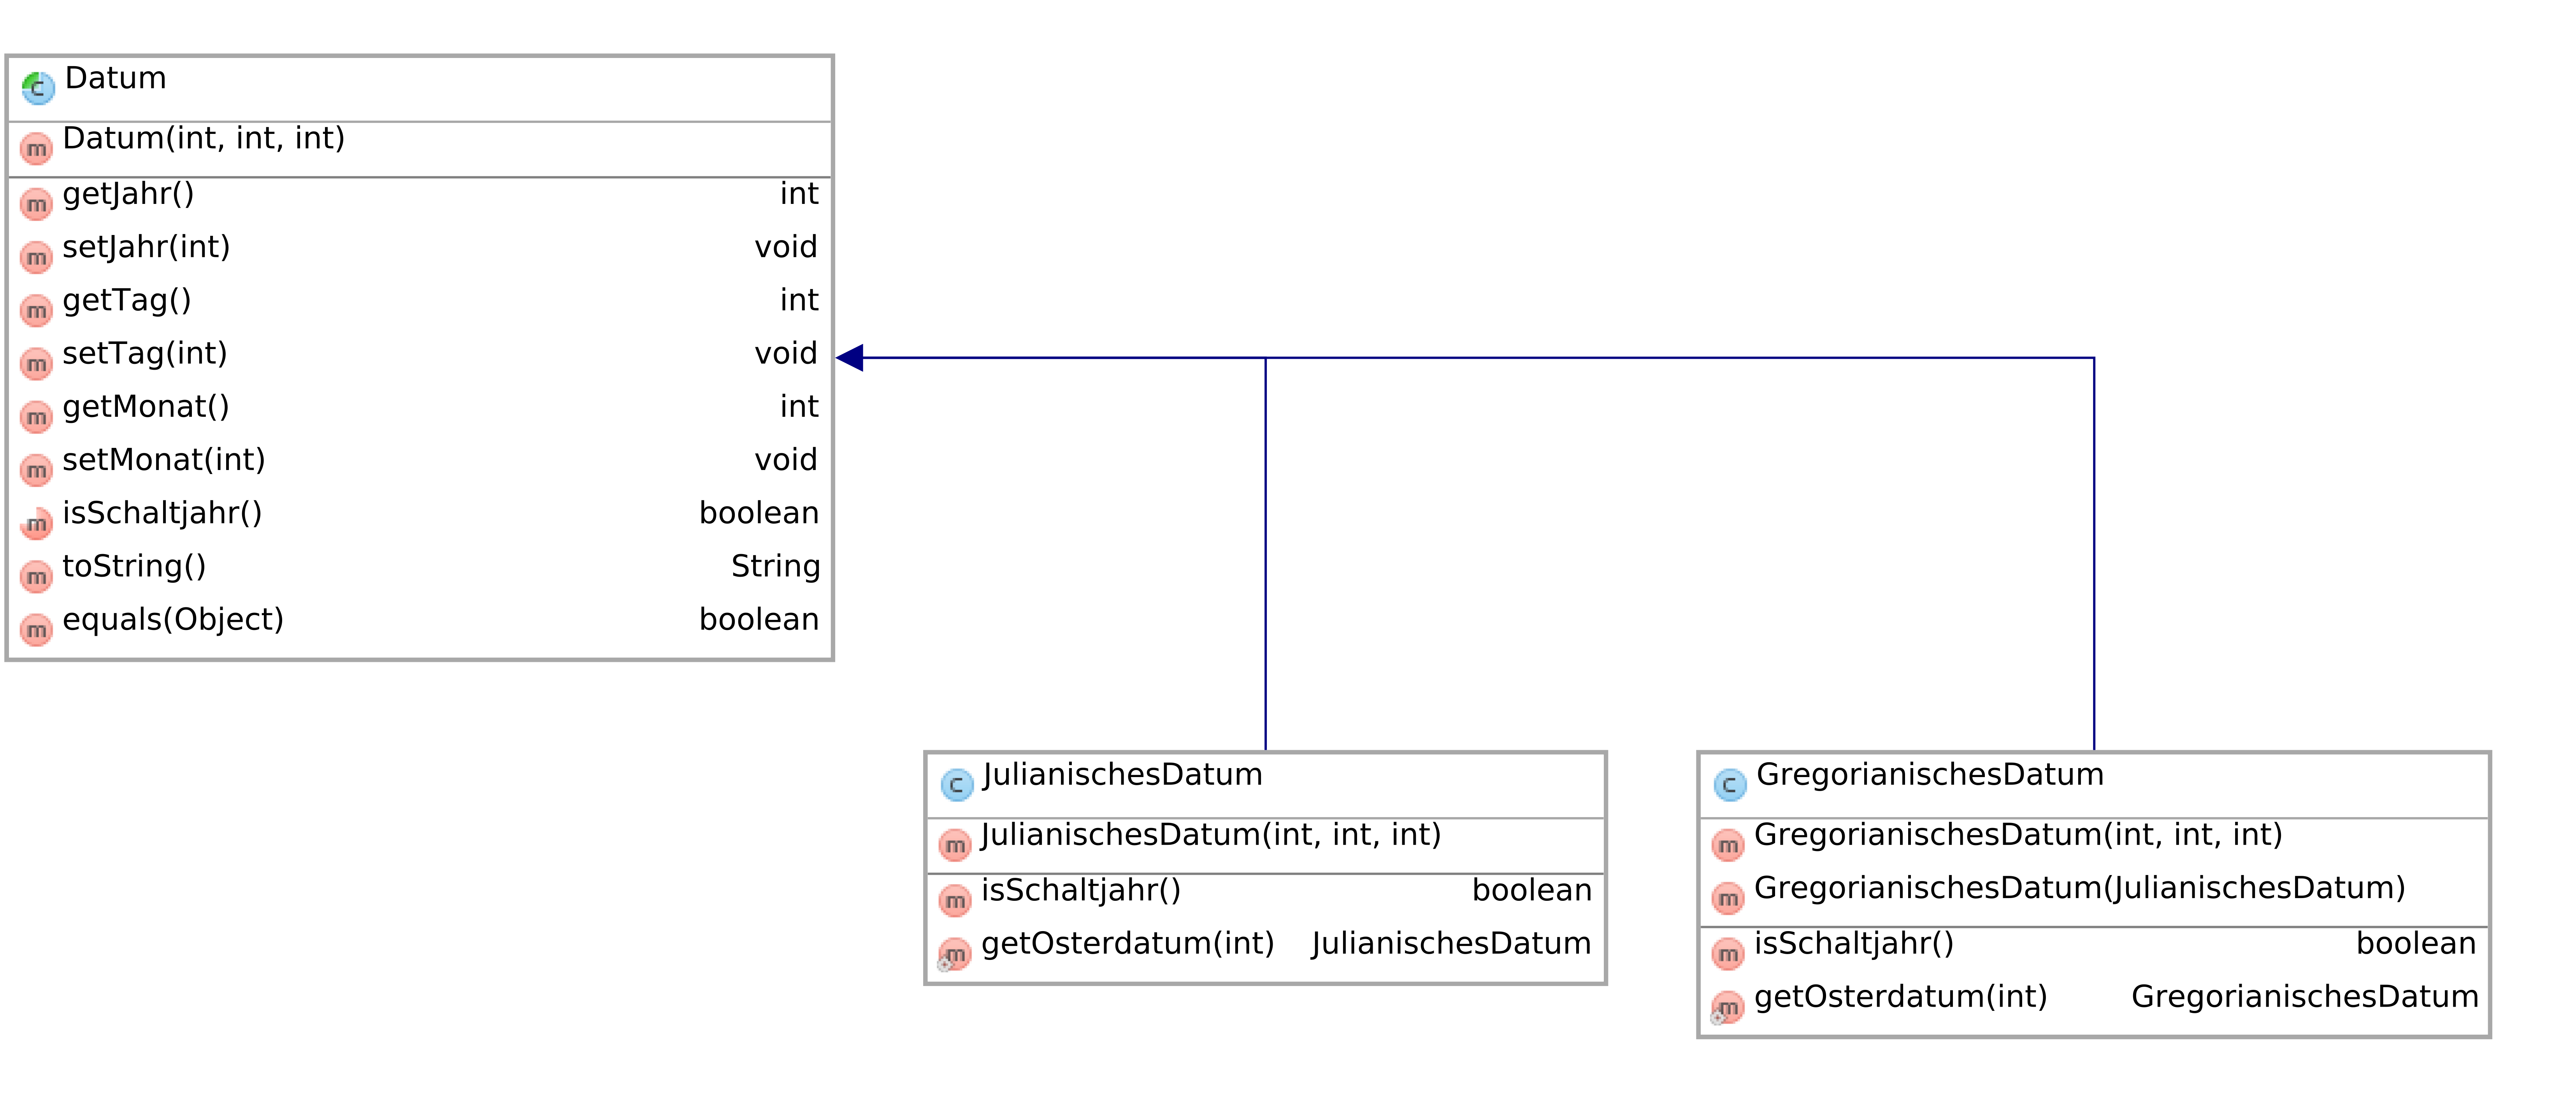
\includegraphics[width=\textwidth]{uml}
	\caption{UML-Diagramm der Implementation}
\end{figure}

Um beide Aufgabenstellungen bearbeiten zu können, muss nun für beide Kalnendersysteme getrennt die Osterformel implementiert werden. Da die Ausgabe im gregorianischen Kalendersystem gefordert wird und Daten verglichen werden müssen, müssen Daten aus dem julianischen Kalender in den gregorianischen Kalender umgerechnet werden können. Dazu gibt es in der gregorianischen Klasse einen überladenen Konstruktor, der ein julianisches Datum entgegennimmt und entsprechend umrechnet.

\clearpage
\subsection{Implementierungen der beiden Kalendersysteme}
	\subsubsection{Implementierung des julianischen Datums}
	Für die Umsetzung des julianischen Datums habe ich das obengenannte Schaltjahrkriterium folgendermaßen nach Java übersetzt:
	\lstinputlisting[firstline=9,lastline=11]{code/datum/JulianischesDatum.java}
	
	Außerdem habe ich die Osterformel von Wikipedia in Java umgesetzt:

	\lstinputlisting[firstline=13,lastline=29]{code/datum/JulianischesDatum.java}
	
	\subsubsection{Implementierung des gregorianischen Datums}

	Auch hier habe ich das Schaltjahkriterium folgendermaßen nach Java übersetzt:
	\lstinputlisting[firstline=14,lastline=16]{code/datum/GregorianischesDatum.java}
	Ebenso habe ich die für den gregorianischen Kalender angepasste Osterformel umgesetzt.
	\lstinputlisting[firstline=18,lastline=35]{code/datum/GregorianischesDatum.java}

	Außerdem gibt es in dieser Klasse noch die Umrechnungsfunktion von dem julianischen in den gregorianischen Kalender. 
	Zunächst wird dabei das julianischem Datum übernommen. Danach wird mit der in der Lösungsidee genannten Formel der Abstand zwischen den beiden Kalendersystemen in dem Jahr des Datums berechnet. Dieser Abstand wird dem Tag hinzuaddiert. Danach wird die Funktion korrigiereUeberhang() aufgerufen. Diese korrigiert das Datum falls durch das hinzuaddieren der Tagesdifferenz die Monatsläge überschritten wurde.

	Zunächst ermittelt diese Funktion die für das Jahr des Datums zutreffenden Monatslängen (Schaltjahr). Danach wird berechnet, um wie viele Tage das gesetzte Datum die Monatslänge des Datums unter-/überschreitet.

	Wenn die Monatslänge überschritten wird, wird folgendermaßen das Datum korrigiert:

	Da die Tage die Monatslänge überschritten haben, muss das Datum mindestens im nächsten Monat liegen. Daher wird der Monat des Datums um eins erhöht. Ist der aktuelle Monat ein Dezember, wird dementsprechend das Jahr um 1 erhöht, der Monat auf Januar gesetzt und der Schaltjahresregel entsprechend die für das neue Jahr gültigen Monatslängen gesetzt.

	Unterschreiten oder gleichen die überhängenden Tage die Monatslänge des neuen Monates, ist die Umrechnung beendet. Die noch überhangenden Tage sind dann der Tag des neuen Monates.

	Überschreiten die überhägenden Tage die Monatslänge des neuen Monates, wird auch dieser Monat, wie zwei Absätze zuvor beschrieben, übersprungen. Die Monatslänge kann von den überhangenden Tagen dann subtrahiert werden.

	Dies wird solange wiederholt, bis das Datum erfolgreich umgerechnet wurde.

	\lstinputlisting[firstline=36,lastline=89]{code/datum/GregorianischesDatum.java}
\clearpage
\subsection{Quelltext Suchcode}
	\lstinputlisting[firstline=14,lastline=39]{code/Main.java}
	\clearpage
	\section{Beispiel}
		Die Programmausgabe lautet:

\shellcmd{java -jar Sprichwort.jar}
\shellout{Kath./Ev. Ostern und Orth. Weihnachten finden am folgendem Datum gleichzeitig statt: 23.3.11919 \\
Kath./Ev. Weihnachten und Orth. Ostern finden am folgendem Datum gleichzeitig statt: 25.12.32839}

Die jeweiligen Lösungen habe ich anschließend mit meinem Taschenrechner überprüft:

	\twocolumn
	\subsection{Kath./Ev. Ostern und Orth. Weihnachten}
		23 März 11919\textsuperscript{gre} / 25. Dez. 11918\textsuperscript{jul}
		\subsubsection{Kath./Ev. Ostern 11919}
			Nach der Gaußschen Osterformel von 1816:
			\begin{align*}
			j &= 11919													\\
			a &= j \bmod 19 = 6											\\
			b &= j \bmod 4 = 3											\\
			c &= j \bmod 7 = 3											\\
			k &= j \div 100 = 119										\\
			p &= (8 \times k + 13) \div 25 = 38							\\
			q &= k \div 4 = 29											\\
			M &= (15 + k - p -q) \bmod 30 = 7							\\
			d &= (19 \times a + M) \bmod 30 = 1							\\
			N &= (4 + k - q) \bmod 7 = 3									\\
			e &= (2 \times b + 4 \times c + 6 \times d + N) \bmod 7 = 0	\\
			O &= 22 + d + e = 23 \text{.März}						
			\end{align*}

			Ostern fällt 11919 auf den 23 März\textsuperscript{gre}!
		\subsubsection{Orthodoxes Weihnachtsdatum 11918}
			Orthodoxes Weihnachtsdatum: 25. Dez. 11918\textsuperscript{jul}. Umrechnung in den gregorianischen Kalender:

			\begin{align*}
			JH &= 119						\\
			a &= JH \div 4 = 29				\\
			b &= JH \bmod 4 = 3				\\
			TD &= 3 \times a + b - 2 = 88 	\\
			\end{align*}

			Vom 25. Dez. 11918 bis zum 1. Jan 11919 sind es 6 Tage, es verbleiben 82 Tage.

			\begin{tabular}{ll}
			Jan 11919: -31                    & R: 51 \\
			Feb 11919: -28 (kein Schaltjahr!) & R: 23
			\end{tabular}

			23 Tage Rest, also liegt der 25. Dez. 11918\textsuperscript{jul} auf dem 23 Mär. 11919\textsuperscript{gre}!
	\newpage
	\subsection{Kath./Ev. Weihnachten und Orthodoxe Ostern}
		25. Dez. 32839\textsuperscript{gre} / 25. Apr. 32839\textsuperscript{jul}
		\subsubsection{Orth. Ostern 32839}
			Nach der Gaußschen Osterformel von 1816:
			\begin{align*}
			j &= 32839														\\	
			a &= j \bmod 19 = 7												\\	
			b &= j \bmod 4 = 3												\\
			c &= j \bmod 7 = 3												\\
			k &= j \div 100 = 328											\\
			M &= (15 + k - p - q) \bmod 30 = 15								\\
			d &= (19 \times a + M) \bmod 30 = 28								\\
			N &= (4 + k - q) \bmod 7 = 6										\\
			e &= (2 \times b + 4 \times c + 6 \times d + N) \bmod 7 = 6		\\
			O &= 22 + d + e = 56\text{.März } \widehat{=} \text{ } 25\text{.Apr}
			\end{align*}

			Osterdatum : 25. Apr. 32839\textsuperscript{jul}

			Umrechnung in den Gregorianischen Kalender:
			\begin{align*}
			JH &= 328						\\
			a &= JH \div 4 = 82				\\
			b &= JH \bmod 4 = 0				\\
			TD &= 3 \times a + b - 2 = 244 	\\
			\end{align*}
			Vom 25. Apr. 32839 bis zum 1. Mai sind es 5 Tage, es verbleiben 239 Tage:

			\begin{tabular}{ll}
				Mai 32839: -31 & R: 208 \\
				Jun 32839: -30 & R: 178 \\
				Jul 32839: -31 & R: 147 \\
				Aug 32839: -31 & R: 116 \\
				Sep 32839: -30 & R: 86  \\
				Okt 32839: -31 & R: 55  \\
				Nov 32839: -30 & R: 25 
			\end{tabular}

			25 Tage Rest, also liegt der 25. Apr. 32839\textsuperscript{jul} auf dem 25. Dez. 32839\textsuperscript{gre}
		\subsubsection{Kath./Ev. Weihnachtsfest 32839}
			32839 findet Weihnachten natürlich am 25. Dez. 32839\textsuperscript{gre} statt.

	\onecolumn
	\clearpage
	\section{Quellcode}
		\subsection{Hauptklasse}
\lstinputlisting {code/Main.java}
\clearpage
\subsection{Datumsklasse}
Ich habe die Oberlasse Datum um Getter- und Settermethoden gekürzt abgedruckt, den Volltext finden Sie im .zip.
\lstinputlisting[firstline=1,lastline=12]{code/datum/Datum.java}
\lstinputlisting[firstline=19,lastline=41]{code/datum/Datum.java}

Die Schaltjahrkriterien sind in der Umsetzung aufgeführt, die Osterformeln sind wie in Wikipedia bei "`Eine ergänzte Osterformel"' beschrieben umgesetzt. Den vollen Quellcode finden Sie im Unterordner "`Sprichwort"'.
\clearpage
\subsection{Umrechnung julianisch \(\rightarrow\) gregorianisch}
\lstinputlisting[firstline=36,lastline=90]{code/datum/GregorianischesDatum.java}

\end{document}